%!TEX encoding = UTF-8 Unicode
\part{Project analysis}

\chapter{User story}

I'm a kid older than 3. I'm in a pre-school or elementary-school age. I
have a tablet computer provided only for educational purposes. I use a
computer mostly at school but I can take it home for the weekend. I may
be not very experienced with computers but I have lots of time, energy
and curiosity. \\

\noindent
I'm using my device in a network set up like: \\*
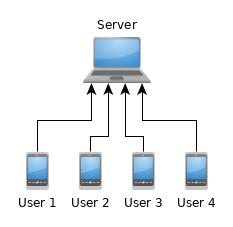
\includegraphics{school.png}


\chapter{Known issues and limitations}

\begin{itemize}
\item The end-user device must be cheaper than \$ 100.
\item The device will work in untrusted environment: at home, for example.
\end{itemize}


\chapter{Goals}

\begin{enumerate}
\item Provide a cheap replaceable device for educational purposes.
\item Determine the project hardware equpment and networking environment.
\end{enumerate}


\chapter{Scope of work}

\section{Requirements}

\begin{enumerate}
\item The end-user device must have a simple rollback functionality for
the cases of incorrect user exploitation.
\item The end-user device must have a limited access to the websites.
\item The end-user device must have application installation
functionality blocked.
\end{enumerate}

\section{Defintion of Done (artifacts)}

\begin{enumerate}
\item Report describing solutions for limiting access to websites and
3rd party software on end-user devices.
\item Provide simple device configuration tutorial in english
\textbf{or} spanish.
\end{enumerate}

